% =============================================================================
% Leveraging LLMs for Data Analysis in Education Research
% EI Fellows Workshop — Stanford SCALE Initiative
% Compile with: pdflatex (twice for refs) or XeLaTeX/LuaLaTeX for true Arial
% =============================================================================
\documentclass[aspectratio=169,t]{beamer}

\usepackage[utf8]{inputenc}
\usepackage[T1]{fontenc}
\usepackage{lmodern}
\usepackage{microtype}
\usepackage{graphicx}
\usepackage{booktabs}

% Load the SCALE theme (beamerthemescale.sty + logo/gear PNGs live alongside
% this file).
\usetheme{scale}

% ---------------------------------------------------------------------------
% Helper: full-width placeholder box for images/screenshots to be added later.
% Usage: \placeholder{height}{caption text}
% ---------------------------------------------------------------------------
\newcommand{\placeholder}[2]{%
  \begin{center}
    \setlength{\fboxsep}{0pt}%
    \fcolorbox{scaleTeal}{scaleLightTeal!20}{%
      \parbox[c][#1][c]{0.8\linewidth}{%
        \centering\itshape\color{scaleGray} [ PLACEHOLDER: #2 ]%
      }%
    }%
  \end{center}%
}

% Application URL used across the interactive sections.
\newcommand{\appurl}{\texttt{https://julian-bernado.github.io/llms4edu/}}

\title{Leveraging LLMs\\for Data Analysis\\in Education Research}
\subtitle{}
\author{Julian Bernado}
\institute{SCALE Initiative, Stanford University}
\date{Thursday, July 16th}

% =============================================================================
\begin{document}

% ---------------------------------------------------------------------------
% 1. Title
% ---------------------------------------------------------------------------
\begin{frame}[plain,noframenumbering]
  \titlepage
\end{frame}

% ---------------------------------------------------------------------------
% 2. Intro to me
% ---------------------------------------------------------------------------
\begin{frame}{About me}
    \vspace{0.5em}
    \begin{itemize}
        \itemsep=1.0em
        \item Stanford Math B.S. (2023), University of Michigan Statistics
              M.A. (2025)
        \item Senior Research Data Analyst here at SCALE (2025-now)
        \item I use natural language processing (NLP) to study
              conversational data
        \item I study what moves tutors use in sessions to engage and teach students
        \item Would love to be a resource for Stanford or post-Stanford life!
    \end{itemize}
\end{frame}

% ---------------------------------------------------------------------------
% 3. Signposting
% ---------------------------------------------------------------------------
\begin{frame}{What we'll do today}

    \begin{block}{The plan}
        I want to show you \textbf{\tealtext{two concrete ways}} to use LLMs when working with data: \textbf{\tealtext{pre-processing}} and \textbf{\tealtext{analysis}}.
    \end{block}
    \vspace{0.5em}
    \begin{alertblock}{My goal}
        You'll come away with both \emph{ideas} for how to use LLMs, some
        \emph{intuition} for why using LLMs requires special attention in
        research, and \textit{experience} using LLMs to process and analyze educational data.
    \end{alertblock}
\end{frame}

% ===========================================================================
\section{Preprocessing}
\roadmapframe
% ===========================================================================

% ---------------------------------------------------------------------------
% 4. Preprocessing: explanation
% ---------------------------------------------------------------------------
\begin{frame}{Preprocessing: from files to tables}
    \begin{itemize}
        \item Often data comes to us as a series of \tealtext{\textbf{unstructured
              files}}.
        \item The data analysis procedures we work with typically want
              something closer to a \tealtext{\textbf{table-like structure}}.
        \item So we're going to dive into turning \textbf{this}\,(1) into
              \textbf{this}\,(2).
    \end{itemize}
    \vspace{0.5em}
    \begin{columns}[c,onlytextwidth]
        \begin{column}{0.44\textwidth}
            \begin{center}
                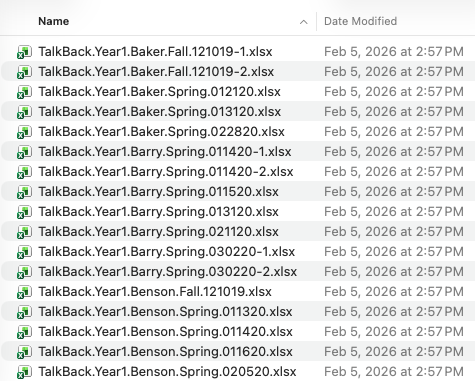
\includegraphics[width=0.9\linewidth]{files.png}
            \end{center}
        \end{column}
        \begin{column}{0.08\textwidth}
            \begin{center}\Large\tealtext{$\longrightarrow$}\end{center}
        \end{column}
        \begin{column}{0.44\textwidth}
            \begin{center}
                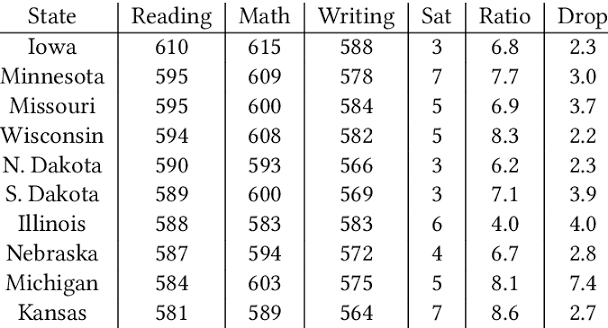
\includegraphics[width=\linewidth]{tabular.png}
            \end{center}
        \end{column}
    \end{columns}
\end{frame}

% ---------------------------------------------------------------------------
% 5. Preprocessing: task description (2 slides)
% ---------------------------------------------------------------------------
\begin{frame}{Preprocessing: the data}
    \begin{itemize}
        \item \tealtext{\textbf{MIT OpenCourseWare}} is a website where you can
              view MIT classes and course materials online.
        \item These are undergraduate and graduate courses from various
              departments at MIT.
        \item I've scraped a \textbf{random sample of 100 syllabi} from MIT OCW.
    \end{itemize}
    \vspace{0.5em}
    \begin{center}
        
\includegraphics[height=2.8cm]{mitocw.png}
    \end{center}
\end{frame}

\begin{frame}{Preprocessing: your task}
    \begin{block}{Goal}
        Build and run a prompt that extracts some \textbf{structured
        information} from these syllabi, then report what you find.
    \end{block}
    Some examples of structured information to extract:
    \begin{itemize}
        \item Does the course have any \textbf{prerequisites}? (True / False)
        \item What percent of the grade comes from
              \textbf{exams / homework / reading / participation}? (number)
        \item How many \textbf{required readings} does the course have? (number)
    \end{itemize}
    \vspace{0.5em}
    \begin{alertblock}{Focus}
        Extract a well-defined \textbf{True/False} value or a \textbf{number}
        from each syllabus.
    \end{alertblock}
\end{frame}

% ---------------------------------------------------------------------------
% 6. Preprocessing: interactive
% ---------------------------------------------------------------------------
\begin{frame}{Preprocessing: your turn}
    \begin{center}
        \Large Go to \appurl
    \end{center}
    \vspace{0.5em}
    \begin{columns}[T,onlytextwidth]
        \begin{column}{0.52\textwidth}
            \textbf{\tealtext{Example research questions}}
            \begin{itemize}
                \item Do courses with prerequisites have more required readings?
                \item How is grade weight distributed across departments?
                \item What share of courses have a final exam?
            \end{itemize}
        \end{column}
        \begin{column}{0.44\textwidth}
            \textbf{\tealtext{Tips}}
            \begin{itemize}
                \item Ask for one well-defined field at a time.
                \item Tell the model exactly what output format you want.
                \item Spot-check a few syllabi by hand.
            \end{itemize}
        \end{column}
    \end{columns}
    \vspace{0.5em}
    \begin{center}
        \small I'll be walking around --- flag me down with questions.
    \end{center}
\end{frame}

% ---------------------------------------------------------------------------
% 7. Preprocessing: discussion
% ---------------------------------------------------------------------------
\begin{frame}{Preprocessing: discussion}
    \begin{block}{Open-ended}
        What did you find? Any reactions to your results?
    \end{block}
    \textbf{\tealtext{Directed questions}}
    \begin{itemize}
        \item Were any of your results \textbf{surprising}?
        \item Did any people measuring the \textbf{same thing} get
              \textbf{different results}?
    \end{itemize}
\end{frame}

% ===========================================================================
\section{Pitfalls}
\roadmapframe
% ===========================================================================

% ---------------------------------------------------------------------------
% 8. Pitfall #1: reproducibility
% ---------------------------------------------------------------------------
\begin{frame}{Pitfall \#1: Reproducibility}
    Different people can run ``the same'' analysis and get different numbers.
    Three common reasons:
    \begin{enumerate}
        \item \textbf{Different models} \\
              {\small Results depend on which model you used --- be transparent
              about model choice.}
        \item \textbf{Benign prompt differences} \\
              {\small Small wording changes can shift results --- track exactly
              which prompt your results came from.}
        \item \textbf{Sampling} \\
              {\small Models are stochastic by default --- set
              \texttt{temperature = 0} for more deterministic output.}
    \end{enumerate}
\end{frame}

% ===========================================================================
\section{Analysis}
\roadmapframe
% ===========================================================================

% ---------------------------------------------------------------------------
% 9. Analysis: explanation
% ---------------------------------------------------------------------------
\begin{frame}{Analysis: interpreting data}
    \begin{itemize}
        \item \tealtext{\textbf{Preprocessing}} uses LLMs to \emph{extract}
              structured information.
        \item \tealtext{\textbf{Analysis}} uses LLMs to \emph{interpret} data.
        \item In reality, the boundary between these two tasks is not always so
              clear.
        \item Now we're going to use LLMs to help us \textbf{understand} our
              data.
    \end{itemize}
\end{frame}

% ---------------------------------------------------------------------------
% 10. Analysis: task description (2 slides)
% ---------------------------------------------------------------------------
\begin{frame}{Analysis: the data}
    \begin{itemize}
        \item These are transcripts from \tealtext{\textbf{classroom
              conversations}} (the \textbf{TalkMoves} dataset).
        \item A common test dataset in the education NLP space.
        \item \textbf{K--12 Mathematics} lessons.
    \end{itemize}
    \vspace{0.5em}
    \begin{center}
        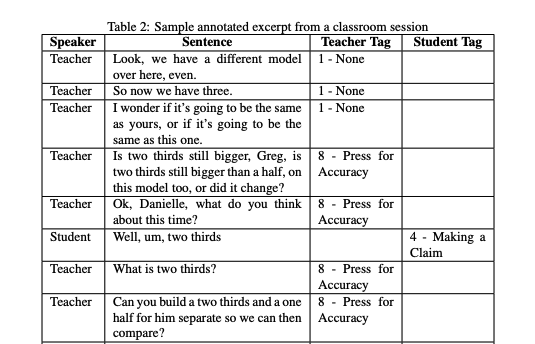
\includegraphics[height=4.5cm]{talkmoves.png}
    \end{center}
\end{frame}

\begin{frame}{Analysis: your task}
    \begin{block}{Goal}
        Imagine you want to understand some \textbf{behavior} in these classroom
        conversations. Write up a description of a behavior --- in teachers or
        students --- that might be present in the transcripts.
    \end{block}
    Some examples of questions to answer:
    \begin{itemize}
        \item \textbf{Praise} after getting a problem correct
        \item Student \textbf{confusion / frustration}
        \item \textbf{Classroom management}
    \end{itemize}
\end{frame}

% ---------------------------------------------------------------------------
% 11. Analysis: interactive
% ---------------------------------------------------------------------------
\begin{frame}{\text{Analysis: your turn}}
    \begin{center}
        \Large Go to \appurl
    \end{center}
    \vspace{0.5em}
    \begin{block}{Prompting tips}
        \begin{itemize}
            \item \textbf{Give examples} of the behavior you're looking for.
            \item Give as much \textbf{context} as possible for what you're
                  trying to do.
            \item \textbf{Read} some transcripts to understand what the
                  conversations look like.
        \end{itemize}
    \end{block}
    \begin{center}
        \small I'll be walking around --- flag me down with questions.
    \end{center}
\end{frame}

% ---------------------------------------------------------------------------
% 12. Analysis: discussion
% ---------------------------------------------------------------------------
\begin{frame}{Analysis: discussion}
    \begin{block}{Open-ended}
        What types of things did people look for?
    \end{block}
    \textbf{\tealtext{Directed questions}}
    \begin{itemize}
        \item Did anybody \textbf{disagree} with the examples the LLM pulled out?
        \item If so, how would you \textbf{modify your prompt} knowing how it
              extracted things?
        \item[$\rightarrow$] If you were reading research studying these
              transcripts, and the outcome was \textbf{annotated by an LLM} this
              way --- what problems do you foresee? What disclaimer would be
              appropriate? What sources of \stanfordred{\textbf{bias}} can we
              imagine?
    \end{itemize}
\end{frame}

% ===========================================================================
\section{Pitfalls}
\roadmapframe
% ===========================================================================

% ---------------------------------------------------------------------------
% 13. Pitfall #2: validity
% ---------------------------------------------------------------------------
\begin{frame}{Pitfall \#2: Validity}
    \begin{itemize}
        \item LLMs can quickly generate \textbf{all} of these annotations.
        \item But how do we know the LLM was \stanfordred{\textbf{right}}?
    \end{itemize}
    \vspace{0.5em}
    \begin{block}{Things to think about doing}
        \begin{itemize}
            \item \textbf{Human validation rounds}
            \item Measuring \textbf{high agreement} (human vs.\ model)
            \item Writing \textbf{unambiguous codebooks}
        \end{itemize}
    \end{block}
\end{frame}

% ---------------------------------------------------------------------------
% 14. Pitfall #3: privacy, pricing
% ---------------------------------------------------------------------------
\begin{frame}{Pitfall \#3: Privacy \& pricing}
    \begin{itemize}
        \item When we use these LLMs, we're calling an \textbf{API} and sending
              our data to a company's servers (OpenAI / Anthropic / Google).
        \item For \stanfordred{\textbf{private data}} --- which some of you may
              be working with --- this can't be freely sent to a company's
              servers.
    \end{itemize}
    \vspace{0.5em}
    \begin{block}{Routes you might use LLMs from}
        \begin{itemize}
            \item \textbf{Direct from an API} --- convenient, but data leaves
                  your control.
            \item \textbf{Sherlock} (or other compute clusters) ---
                  institutional, more control.
            \item \textbf{Locally} --- data never leaves your machine.
        \end{itemize}
    \end{block}
\end{frame}

% ===========================================================================
\section{Takeaways}
\roadmapframe
% ===========================================================================

% ---------------------------------------------------------------------------
% 15. Takeaways
% ---------------------------------------------------------------------------
\begin{frame}{Takeaways}
    \begin{columns}[T,onlytextwidth]
        \begin{column}{0.48\textwidth}
            \textbf{\tealtext{Two use cases}}
            \begin{enumerate}
                \item Preprocessing
                \item Analysis
            \end{enumerate}
        \end{column}
        \begin{column}{0.48\textwidth}
            \textbf{\tealtext{Three pitfalls}}
            \begin{enumerate}
                \item Reproducibility
                \item Validity
                \item Privacy \& pricing
            \end{enumerate}
        \end{column}
    \end{columns}
    \vspace{1em}
    \begin{alertblock}{Closing question}
        Can you imagine using LLMs in your work this summer, or in the stuff
        you're interested in? What kinds of questions could it let you answer?
        (All good if not!)
    \end{alertblock}
\end{frame}

% ---------------------------------------------------------------------------
% Closing
% ---------------------------------------------------------------------------
\closingframe{Thanks!}{}

\end{document}
